% Physics experiment report
% 23/Sep/2016

\documentclass[a4paper,10pt,notitlepage]{report}

\usepackage{CJKutf8}
\usepackage{amsmath}
\usepackage{indentfirst}
\usepackage{graphicx}

\setlength{\parindent}{2em} 

\begin{CJK*}{UTF8}{gbsn}
\begin{document}

\title{测量薄透镜焦距实验报告}
\author{秦光辉}
\maketitle

\section*{一、实验数据处理}
\subsection*{1.位移法测凸透镜焦距}

	使用位移法测量凸透镜焦距的时候我一共测得了三组数据,列于表一.如图一所示,$x_1$是物的坐标.$x_2$是屏的位置,$x_3$是成小像的时候凸透镜的坐标,$x_4$是成大像的时候凸透镜的坐标.f是凸透镜焦距,A与l计算公式如式(1)与式(2),f计算公式见式(3).\\
	
\begin{align}
	A=| x_1 - x_2 | \\
	l=| x_3 - x_4 | \\
	f=\frac{A^2 - l^2}{4A} 
\end{align}
	
\begin{figure}[htbp]
\centering

	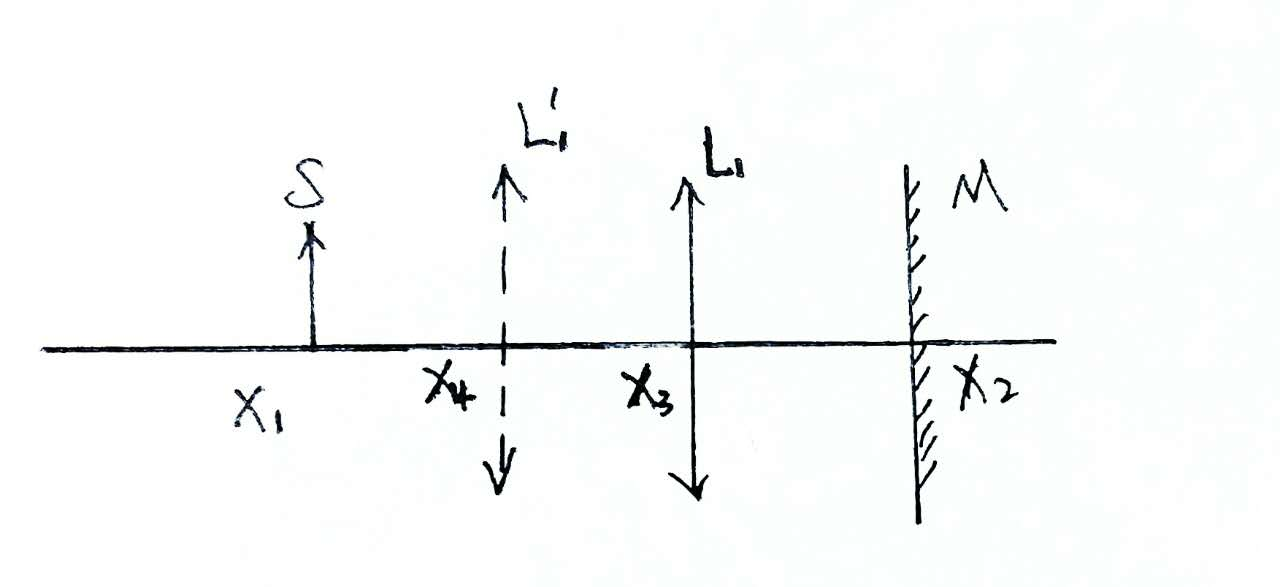
\includegraphics[bb=0 0 1280 587,scale=.15]{wyt.jpg}
	\begin{center}
		\scriptsize Figure 1 位移法测凸透镜焦距光路图
	\end{center}

\end{figure}
	
\begin{table}[htbp]
\centering
	\begin{tabular}{|l|l|l|l|l|l|l|l|}
	
		\multicolumn{1}{l}{\scriptsize unit:cm} \\
		\hline
		次数 & $x_1$ & $x_2$ & A & $x_3$ & $x_4$ & l & f \\
		\hline
		1 & 152.34 & 87.97 & 64.37 & 129.22 & 110.61 & 18.61 & 14.75 \\
		\hline
		2 & 152.34 & 89.80 & 62.54 & 128.57 & 113.25 & 15.32 & 14.70 \\
		\hline
		3 & 152.34 & 91.41 & 60.93 & 127.65 & 116.55 & 11.10 & 14.73 \\
		\hline
		\multicolumn{8}{c}{\scriptsize Table 1\ 位移法测凸透镜焦距数据表} \\

	\end{tabular}
\end{table}

	三次实验数据比较接近,取平均得

\begin{equation}
	\bar{f} = 14.73 cm
\end{equation}

\subsection*{2.物像距法测凹透镜焦距}

	物像距法测凹透镜焦距的实验一共得到了3组数据,列于表二.如图二所示,$x_1$为第一次成像坐标,$x_2$是凹透镜坐标,$x_3$是第二次成像坐标.f是凹透镜坐标,如式(5)所示,可以用上述数据获得f.
	
\begin{equation}
	f=\frac{-1}{\frac{1}{x_1 - x_2} + \frac{1}{x_2 - x_3}} \\
\end{equation}

\begin{figure}[htbp]
\centering

	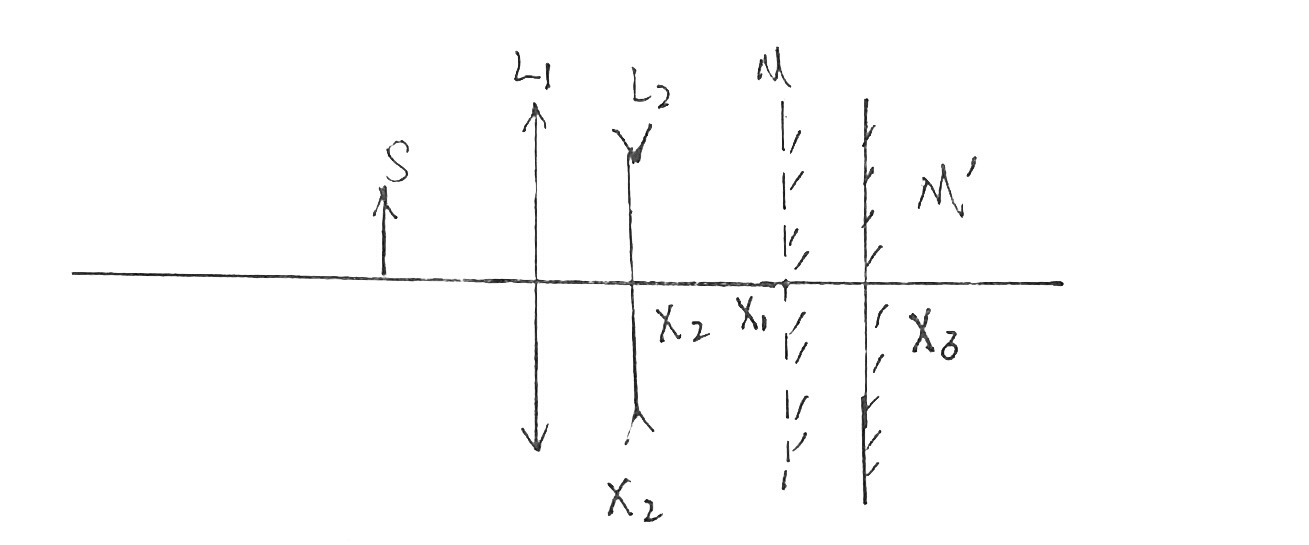
\includegraphics[bb=0 0 1309 545,scale=.15]{wxa.jpg}
	\begin{center}
		\scriptsize Figure 2 物像距法测凹透镜焦距光路图
	\end{center}

\end{figure}

\begin{table}[htbp]
\centering
	\begin{tabular}{|l|l|l|l|l|}

		\multicolumn{1}{l}{\scriptsize unit:cm} \\
		\hline
		\# & $x_1$ & $ x_2$ & $x_3$ & f \\
		\hline
		1 & 88.40 & 97.89 & 66.57 & 13.62 \\
		\hline
		2 & 89.32 & 99.05 & 66.30 & 13.84 \\
		\hline
		3 & 87.88 & 96.83 & 71.19 & 13.74 \\
		\hline
		\multicolumn{5}{c}{\scriptsize Table 2\ 物像距法测凹透镜焦距实验数据} \\
	
	\end{tabular}
\end{table}

	对上述结果取均值有
	
\begin{equation}
	\bar{f}=13.73cm
\end{equation}

\subsection*{3.自准直法测凸透镜焦距}

	自准直法测凸透镜焦距只测了一组数据,如表三所示.如图三所示,表中$x_1$表示物的位置,$x_2$表示凸透镜的位置,$x_3$表示反射平面镜的位置.f表示凸透镜的焦距,其计算公式见式(7).
	
\begin{equation}
	f=|x_1 - x_2| \\
\end{equation}
	
\begin{figure}
\centering

	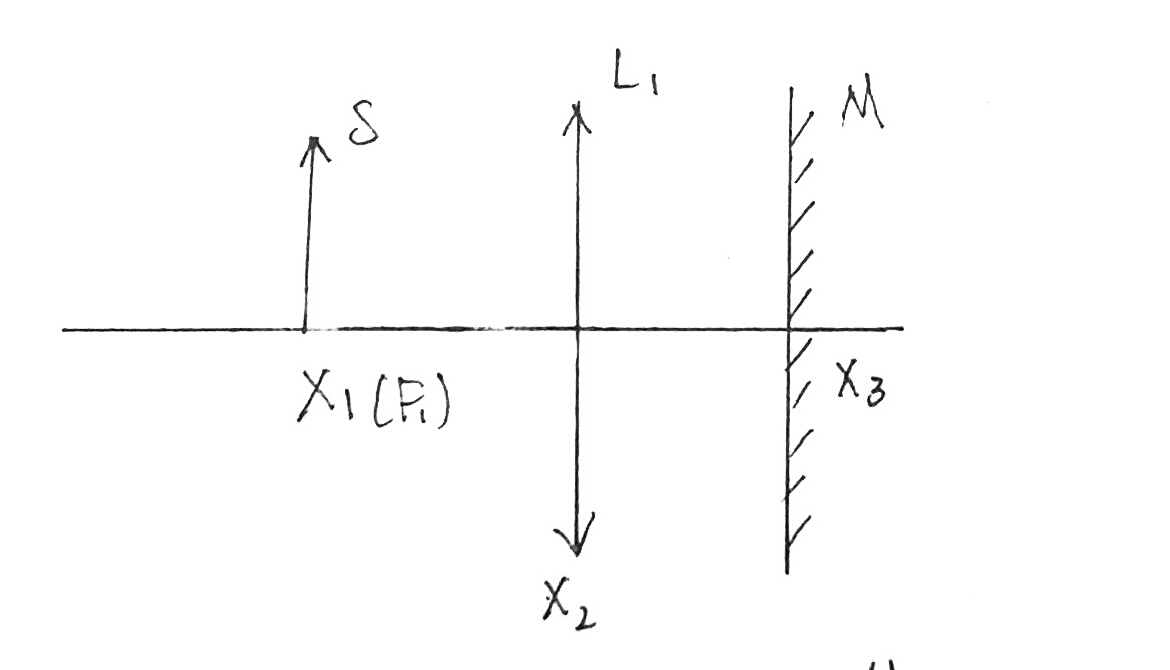
\includegraphics[scale=0.1]{zzt.jpg}
	\begin{center}
		\scriptsize Figure 3\ 自准直法测凸透镜焦距光路图
	\end{center}
	
\end{figure}

\begin{table}[htbp]
\centering
\begin{tabular}{|l|l|l|l|}

	\multicolumn{1}{l}{\scriptsize unit:cm} \\
	\hline
	$x_1$ & $x_2$ & $x_3$ & f \\
	\hline
	152.34 & 137.68 & 117.66 & 14.66 \\
	\hline
	\multicolumn{4}{c}{\scriptsize Table 3\ 自准直法测凸透镜焦距数据表} \\

\end{tabular}
\end{table}

	用自准直法测得凹透镜焦距为14.66cm.

\subsection*{4.自准直法测凹透镜焦距}

	自准直法测凹透镜焦距实验也只获得了一组数据,如表4所示.如图4所示,表4中$x_1$表示第一次成像位置,$x_2$表示凹透镜位置,$x_3$表示反射平面镜位置.f是凹透镜焦距,计算公式见式(8).
	
\begin{equation}
	f=|x_1 - x_2| \\
\end{equation}

\begin{figure}
\centering

	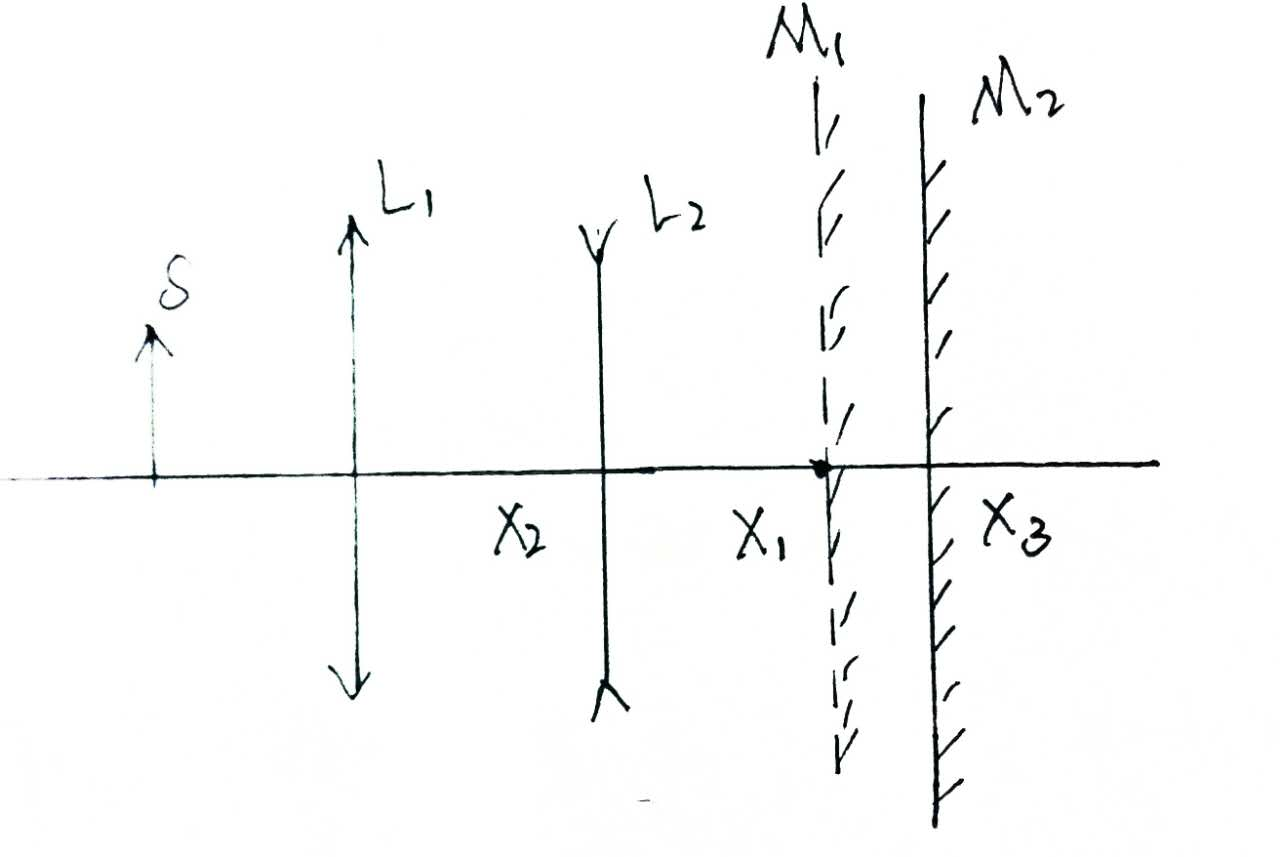
\includegraphics[scale=0.1]{zza.jpg}
	\begin{center}
		\scriptsize Figure 4\ 自准直法测凹透镜焦距光路图
	\end{center}

\end{figure}

\begin{table}[htbp]
\centering
\begin{tabular}{|l|l|l|l|}

	\multicolumn{1}{l}{\scriptsize unit:cm} \\
	\hline
	$x_1$ & $x_2$ & $x_3$ & f \\
	\hline
	86.67 & 100.52 & 87.30 & 13.85 \\
	\hline
	\multicolumn{4}{c}{\scriptsize Table 4\ 自准直法测凹透镜焦距数据表} \\

\end{tabular}
\end{table}
			
	自准直法测的凹透镜焦距为13.85cm.

\section*{二、分析和讨论}
\subsection*{1.位移法和自准直法优缺点分析}
	
	自准直法相对于位移法而言,实验步骤简单,计算也相对简单,可以迅速得到结果,但是并不精确,在焦距附近1cm范围内我们都能看到成像.而且如果光学元件的中心没有对准滑块上的中心的话会带来较大的误差.
	
	位移法计算相对复杂,需要两次成像,由于多次测量也难免带来对准误差,但是位移法实验中A与l的测定都是坐标的差值,这样我们可以避免由于光学元件中心和滑块中心没有对准而产生误差.如果A取值合理的话,位移法的两次成像景深也很很短,这样我们就能比较精确的测得凸透镜焦距.
	
\subsection*{2.误差来源分析}

\begin{enumerate}
	\item 由于读数上的偏差而产生的对准误差
	\item 成像景深较大时产生的误差
	\item 如果没有完全共轴,光路和标尺不平行,带来误差
	\item 光学元件没有完全居中带来的读数误差
\end{enumerate}

\section*{三、感悟和收获}

	光具座上的光学实验是我做的第一个普通物理实验.通过这次实验,我第一次认识到原来物理不只有枯燥乏味的公式推导,而且有很多充满未知数的实验.实验中遇到了很多问题,比如很难调到共轴,比如凹透镜成像很不清晰,无法读数等.做完实验以后感觉很有成就感,虽然数据并不非常精确,但是非常难得.希望自己以后能享受实验的过程,而不囿于数据的好坏.
	
	另外我发现,不能着急动手.共轴和实验方案等,都必须事先想好,不然到时候手忙脚乱,最后数据特别糟糕的时候,还得回到起点重新做.比如我用自准直测凹透镜焦距的时候一直让凸透镜成大像,这样透过凹透镜的光线会非常微弱,后来我听了老师建议换成小像,才完成了实验.所以一定要耐心做好准备才能动手!

\end{CJK*}
\end{document}

